\chapter{СВЕРТОЧНЫЕ НЕЙРОННЫЕ СЕТИ ДЛЯ ДЕТЕКТИРОВАНИЯ}

\section{Сверточные нейронные сети}

%Распознавание и классификация изображений достаточно успешно осуществляются с помощью сверточных нейронных сетей. Нейронная сеть – это некоторая математическая модель, которая состоит из соединенных между собой искусственных нейронов . Сеть принимает в качестве входных данных вектор признаков, затем последовательно пропускает их через слои сети. На выходе получаются вероятности принадлежности объекта к заданным классам. Обычно нейронная сеть оперирует числовыми, а не символьными величинами.

Сеть свертки представляет собой многoслойный персептрон -- математическая или компьютерная модель восприятия информации мозгом, созданный для распознавания 2D-поверхностей с высокой степенью устойчивости к масштабированию, преобразованиям и другим видам деформации. Обучение решению такой задачи осуществляется с подкреплением, при этом используются сети вида, архитектура которых соответствует следующим ограничениям .

Каждый нейрон получает входной сигнал от локального рецептивного поля в предыдущем слое, извлекая его локальные признаки. Как только признак извлечен, его местоположение не имеет значения, т.к. приблизительно установлено его расположение относительно других признаков.

Каждый вычислительный слой сети состоит из множества карт признаков. Каждая карта признаков имеет форму плоскости, на которой все нейроны должны совместно использовать одно и то же множество синаптических весов. Эта форма структурных ограничений имеет преимущества.

За каждым слоем свертки следует вычислительный слой, осуществляющий локальное усреднение (local averaging) и подвыборку (subsampling). Посредством локального усреднения достигается уменьшение разрешения для карт признаков. Такая операция приводит к уменьшению чувствительности выходного сигнала оператора отображения признаков, а также к смещению и другим формам преобразований.


\section{Алгоритм YOLOv3}

YOLO  – это сверточная нейронная сеть, позволяющая одновременно детектировать и классифицировать. Для решения этой задачи предыдущие способы использовали конвейерную обработку, которая включала в себя несколько этапов. Из-за особенностей архитектуры и необходимости обучать каждый отдельный компонент, эти методы достигали малой производительности и были сложны в оптимизации. YOLO избегает этих проблем, сводя задачу обнаружения объектов к простой регрессии. Этот алгоритм одновременно как предсказывает положение и размеры прямоугольников вокруг объектов, так и класс предметов. В отличие от алгоритмов, которые используют принцип скользящего окна, YOLO использует все изображение. 

\begin{figure}
	\centering
	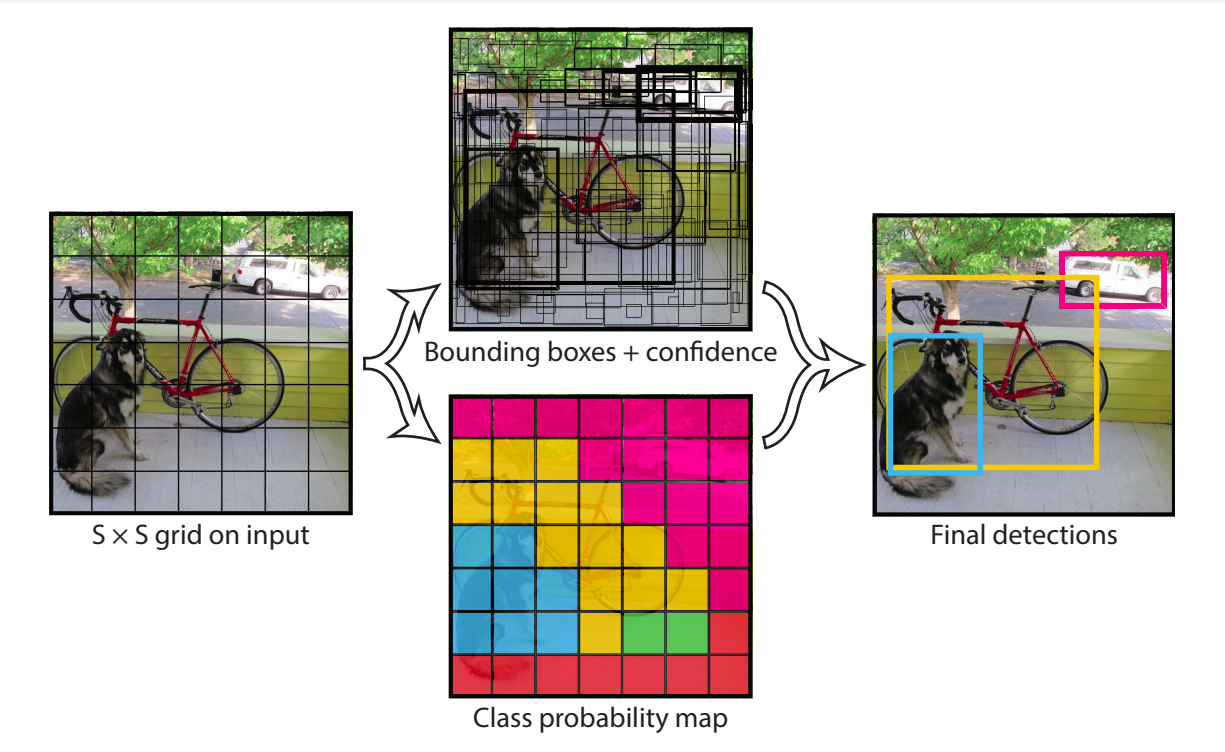
\includegraphics[width=0.7\linewidth]{images/process}
	\caption{Принцип работы алгоритма}
	\label{fig:process}
\end{figure}



В общем, алгоритм принимает на вход изображение, уменьшает размер до $416 \times 416$, пропускает через нейронную сеть (близкую по структуре к сверхточной), которая возвращает результирующий вектор. Более подробное описание можно найти в оригинальной статье. (You Only Look Once:
Unified, Real-Time Object Detection [https://arxiv.org/abs/1506.02640])

% картинка отсюда https://www.researchgate.net/publication/335228064_Deep_Neural_Network-Based_Robust_Ship_Detection_Under_Different_Weather_Conditions

\begin{figure}
	\centering
	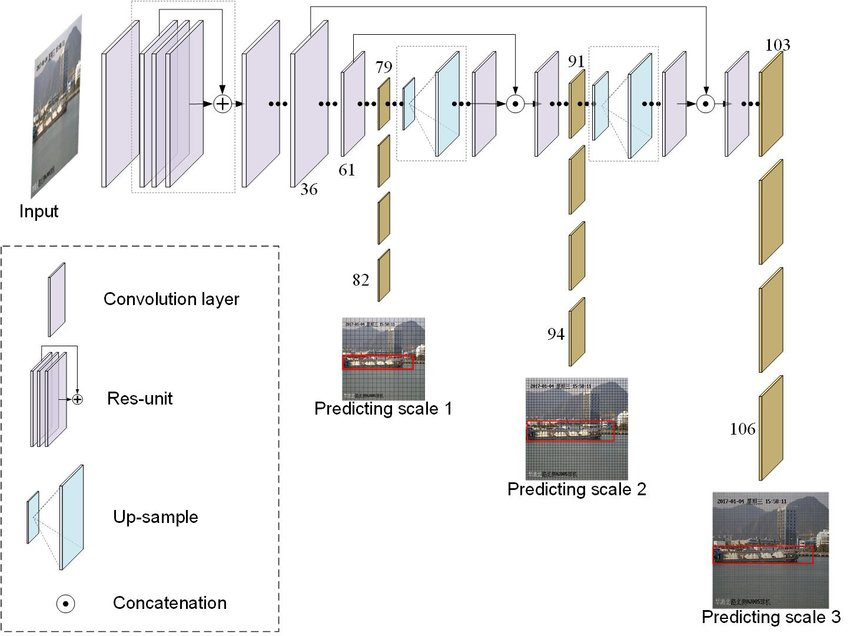
\includegraphics[width=0.8\linewidth]{yolo-structure}
	\caption{Структура нейронной сети.}
	\label{fig:the-framework-of-yolov3-neural-network-for-ship-detection}
\end{figure}

Результирующий вектор \eqref{eqn:output_vector} состоит из следующих параметров:

\begin{itemize}
	\item $p_c$ -- вероятность того, что прямоугольник содержит обнаруживаемый объект
	\item параметры прямоугольника: прямоугольные координаты ($b_x$, $b_y$), ширина ($b_w$), высота ($b_h$)
	\item $c_1, c_2, c_3, ..., c_n$ -- вероятности классов
\end{itemize}

\begin{equation}
Y = [p_c, b_x, b_y, b_h, b_w, c_1, c_2, c_3, ..., c_n]
\label{eqn:output_vector}
\end{equation}

\begin{figure}
	\centering
	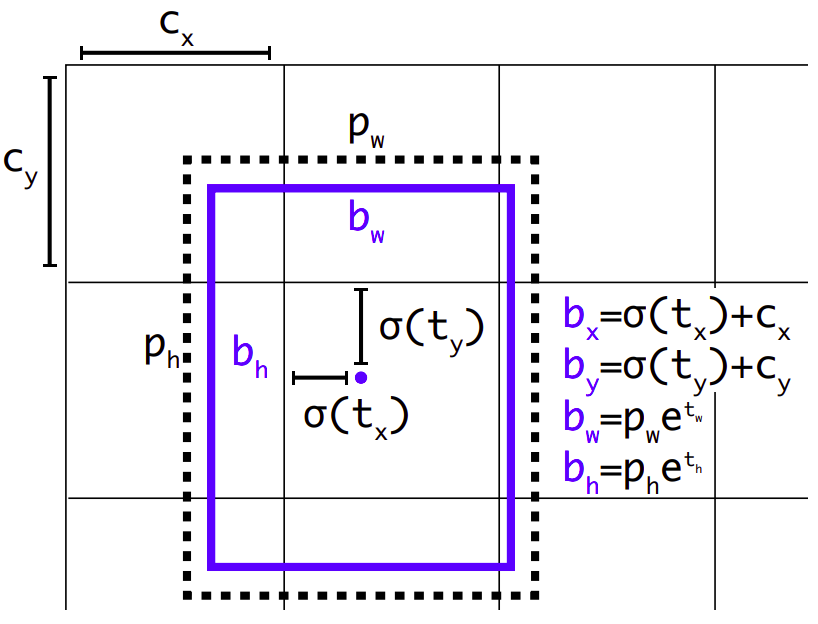
\includegraphics[width=0.7\linewidth]{images/bounding-boxes}
	\caption{}
	\label{fig:bounding-boxes}
\end{figure}


%
%\end{equation}
%
%\begin{multline}
%	\lambda_\textbf{coord}
%	\sum_{i = 0}^{S^2}
%	\sum_{j = 0}^{B}
%	\mathlarger{\mathbbm{1}}_{ij}^{\text{obj}}
%	\left[
%	\left(
%	x_i - \hat{x}_i
%	\right)^2 +
%	\left(
%	y_i - \hat{y}_i
%	\right)^2
%	\right]
%	\\
%	+ \lambda_\textbf{coord} 
%	\sum_{i = 0}^{S^2}
%	\sum_{j = 0}^{B}
%	\mathlarger{\mathbbm{1}}_{ij}^{\text{obj}}
%	\left[
%	\left(
%	\sqrt{w_i} - \sqrt{\hat{w}_i}
%	\right)^2 +
%	\left(
%	\sqrt{h_i} - \sqrt{\hat{h}_i}
%	\right)^2
%	\right]
%	\\
%	+ \sum_{i = 0}^{S^2}
%	\sum_{j = 0}^{B}
%	\mathlarger{\mathbbm{1}}_{ij}^{\text{obj}}
%	\left(
%	C_i - \hat{C}_i
%	\right)^2
%	\\
%	+ \lambda_\textrm{noobj}
%	\sum_{i = 0}^{S^2}
%	\sum_{j = 0}^{B}
%	\mathlarger{\mathbbm{1}}_{ij}^{\text{noobj}}
%	\left(
%	C_i - \hat{C}_i
%	\right)^2
%	\\
%	+ \sum_{i = 0}^{S^2}
%	\mathlarger{\mathbbm{1}}_i^{\text{obj}}
%	\sum_{c \in \textrm{classes}}
%	\left(
%	p_i(c) - \hat{p}_i(c)
%	\right)^2
%\end{multline}


\chapter{АРХИТЕКТУРА СИСТЕМЫ}


\section{Получение информации}


Система получает изображение с камеры видеонаблюдения. Предполагается, что камера установлена под некоторым фиксированным углом, а кадры выровнены в горизонтальной плоскости. 

\section{Калибровка}

Для вычисления расстояния нам необходимо сопоставить координаты на изображении и в реальном мире. Для этого мы используем инструмент калибровки.


В процессе калибровки мы запрашиваем у пользователя координаты квадрата на изображении, все точки которого располагаются на плоскости, параллельной земле. 


\begin{figure}[H]
    \centering
    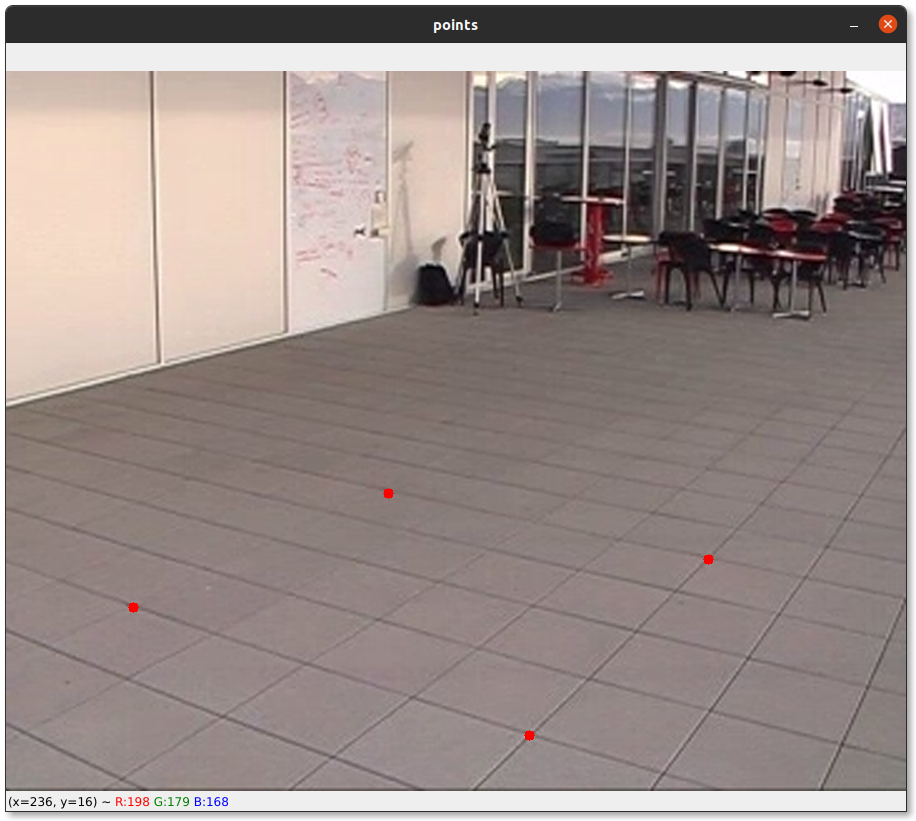
\includegraphics[width=10cm]{images/calibration1.png}
    \caption{Калибровка. Выбираем 4 точки квадрата на изображении}
    \label{<label>}
\end{figure}

Далее у пользователя запрашивается желаемый масштаб и смещение. Преобразования производятся при помощи матрицы гомографии.

Для получения матрицы используется метод OpenCV getPerspectiveTransform. В качестве параметров он принимает 4 координаты из входного и выходного изображения. Далее при помощи полученных значений кадр преобразуется в ''вид сверху'', а также с их помощью вычисляются  расстояния между людьми.


\begin{figure}[H]
    \centering
    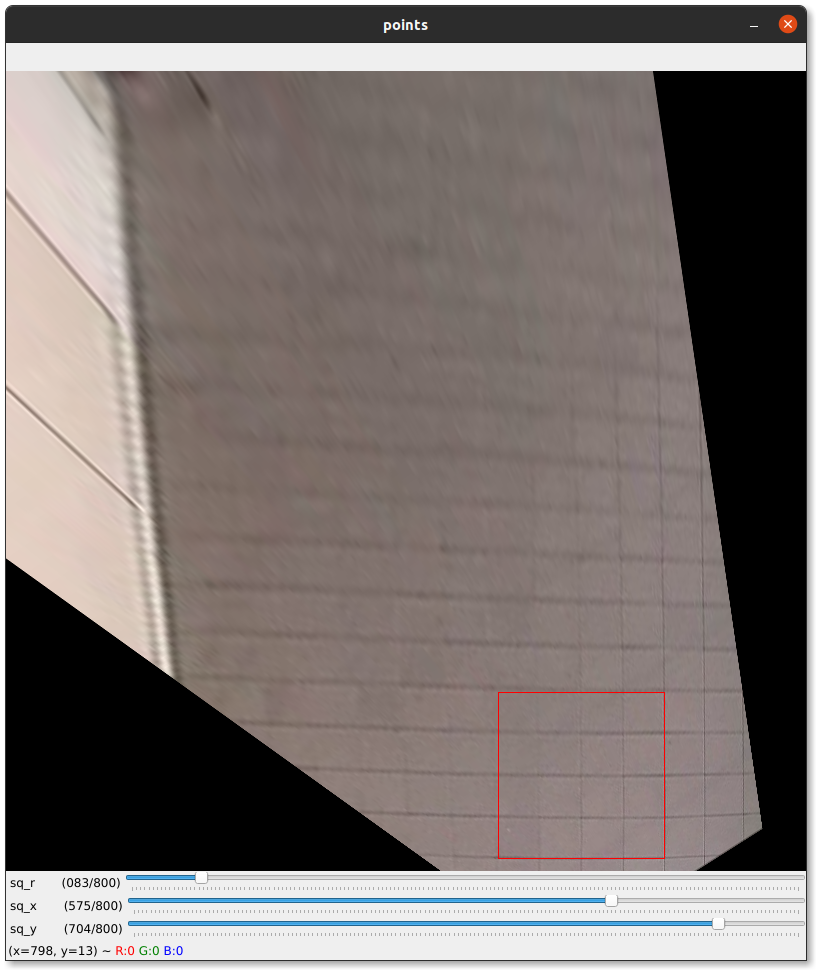
\includegraphics[width=10cm]{images/calibration2.png}
    \caption{Калибровка. Выбираем желаемый масштаб и смещение}
    \label{<label>}
\end{figure}


\section{Обнаружение людей}

Для обнаружения на изображении людей используется система распознавания YOLO. Мы используем уже обученную модель. Нейронная сеть обучалась на датасете Common Object in Context (COCO), который включает 80 категорий объектов, в том числе и людей.

%Модель глубоких сверточных нейронных сетей - это простая и эффективная модель для обнаружения объектов. Эта модель рассматривает регион, который содержит только класс "Человек", и отбрасывает регионы, которые, скорее всего, не содержат никаких объектов. Этот процесс выделения регионов, которые содержат только объекты, называется "Предложения регионов". Регионы, предсказанные с помощью предложения регионов, могут быть разного размера и перекрываться с другими регионами. Поэтому для игнорирования границ, окружающих перекрывающийся регион, в зависимости от показателя Intersection Over Union (IOU) используется максимальное неподавление.


 Мы передаем на вход изображение, а на выходе получаем координаты прямоугольников вокруг объектов, их класс и вероятность принадлежности к нему. 


\section{Вычисление расстояния}

По полученным координатам прямоугольников найдем координаты центральной точки на нижней грани. При помощи матрицы преобразования перспективы, отображаем координаты этих точек на плоскость (вид сверху).

\begin{figure}[H]
    \centering
    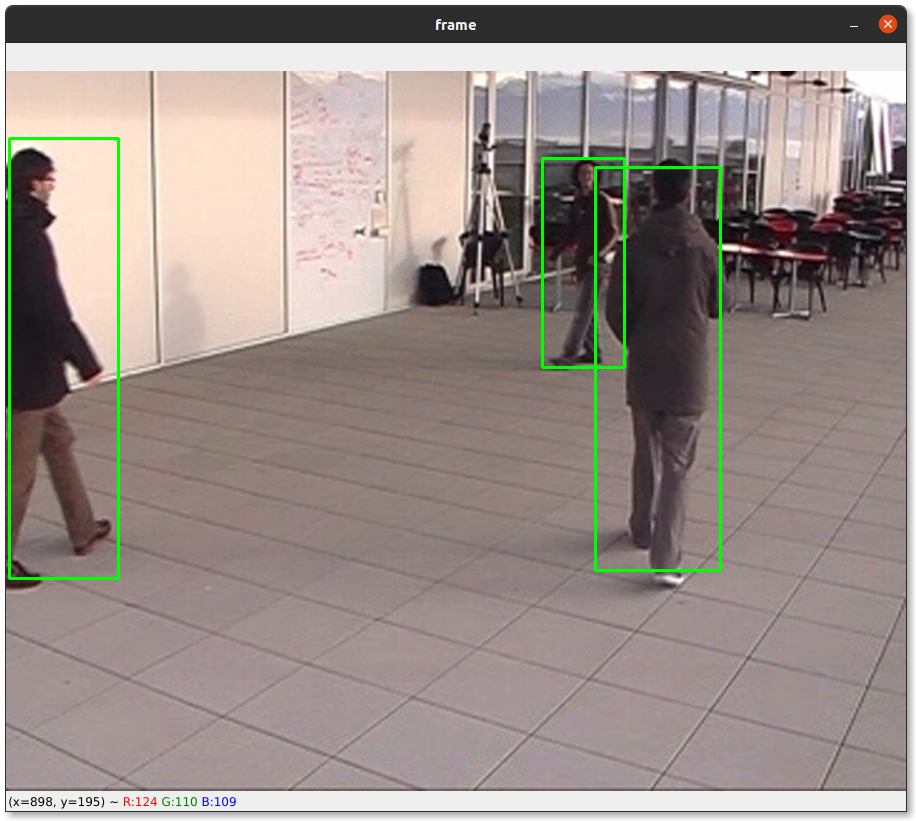
\includegraphics[width=10cm]{images/safe1.png}
    \caption{Зеленым отмечены люди на безопасной дистанции друг от друга}
    \label{<label>}
\end{figure}

Далее перебираем все возможные пары точек и вычисляем для них евклидово расстояние по проекции. Если расстояние меньше определенного значения, помечаем координату.

\begin{figure}[H]
    \centering
    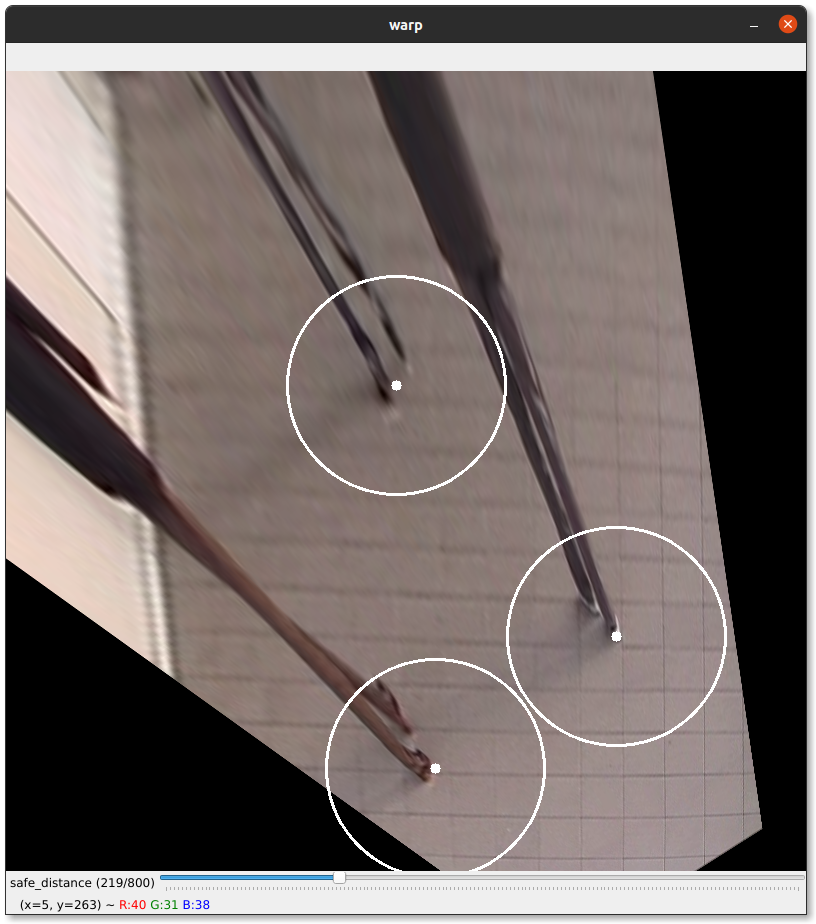
\includegraphics[width=10cm]{images/safe2.png}
    \caption{Вид сверху}
    \label{<label>}
\end{figure}

Рисуем на виде сверху окружности соответствующие безопасной дистанции, а на основном изображении, в зависимости от расстояния до других людей, рамку вокруг человека зеленого или красного цвета.

\begin{figure}[H]
    \centering
    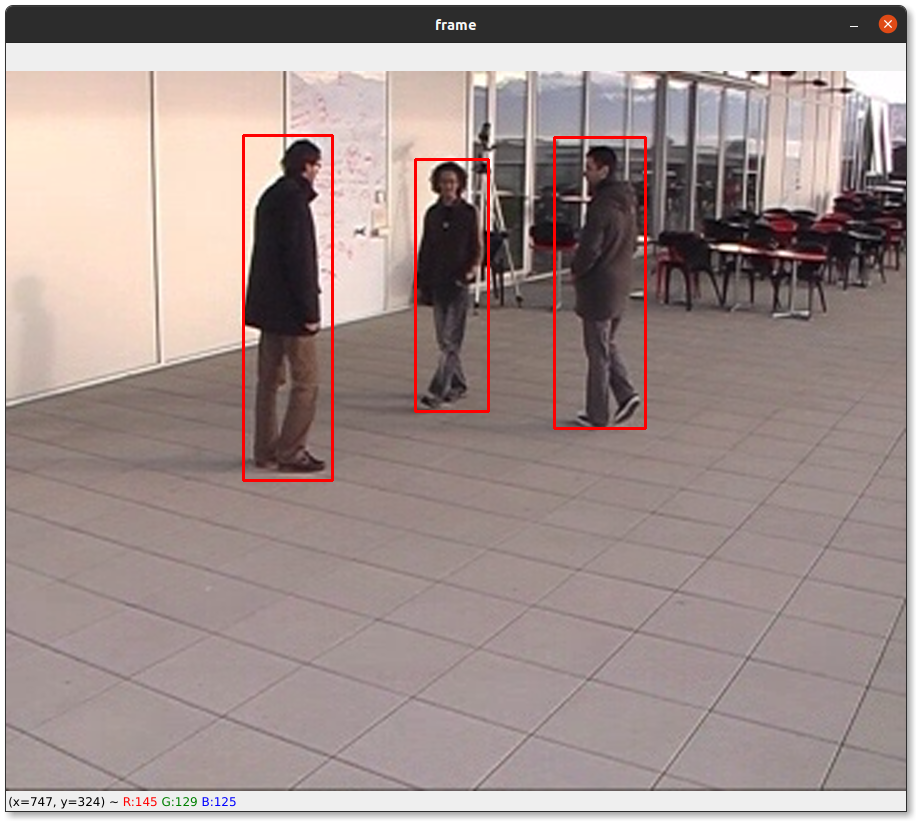
\includegraphics[width=10cm]{images/danger1.png}
    \caption{Красным отмечены люди, нарушающие социальную дистанцию}
    \label{<label>}
\end{figure}

\begin{figure}[H]
    \centering
    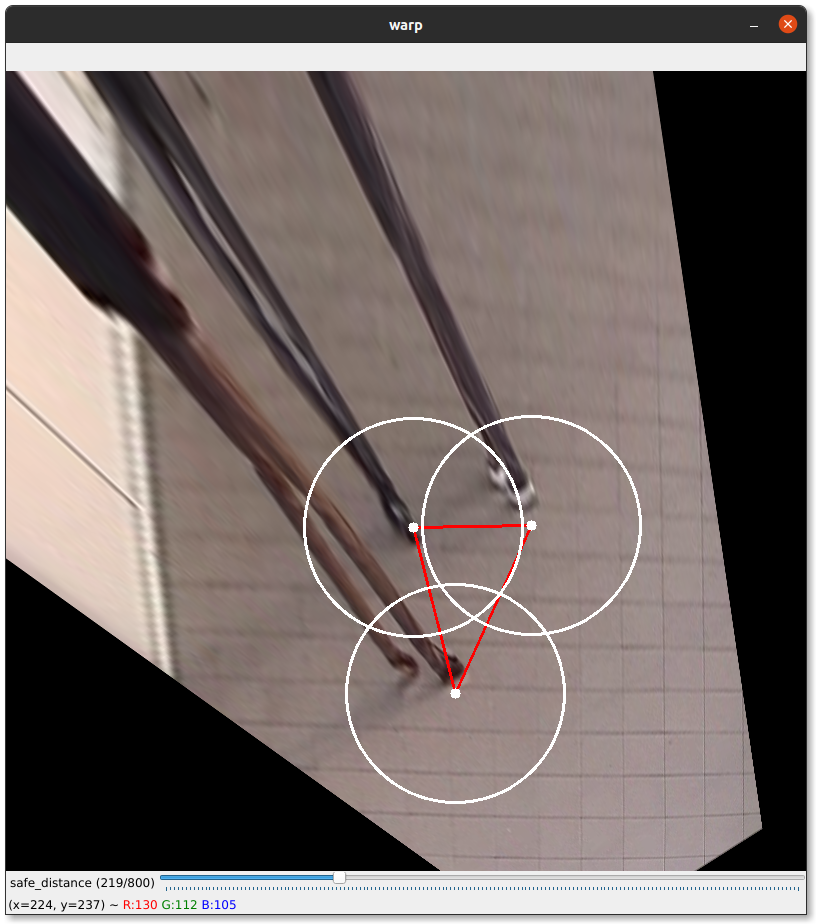
\includegraphics[width=10cm]{images/danger2.png}
    \caption{Вид сверху}
    \label{<label>}
\end{figure}
